The figures in this section show the projected statistical asymmetry uncertainties $\Delta A_{1n}^h$ for five hadron species ($\pi^+$, $\pi^-$, $\pi^0$, $K^+$, $K^-$) at 11 and 8.8 GeV beam energies in two-dimensional $(x,z)$ bins. For more details including numerical tables of projected asymmetry uncertainties and numbers of events for 1D, 2D and 3D kinematic binning, see~\cite{Projections_link}.   

\begin{figure}[h]
  \begin{center}
    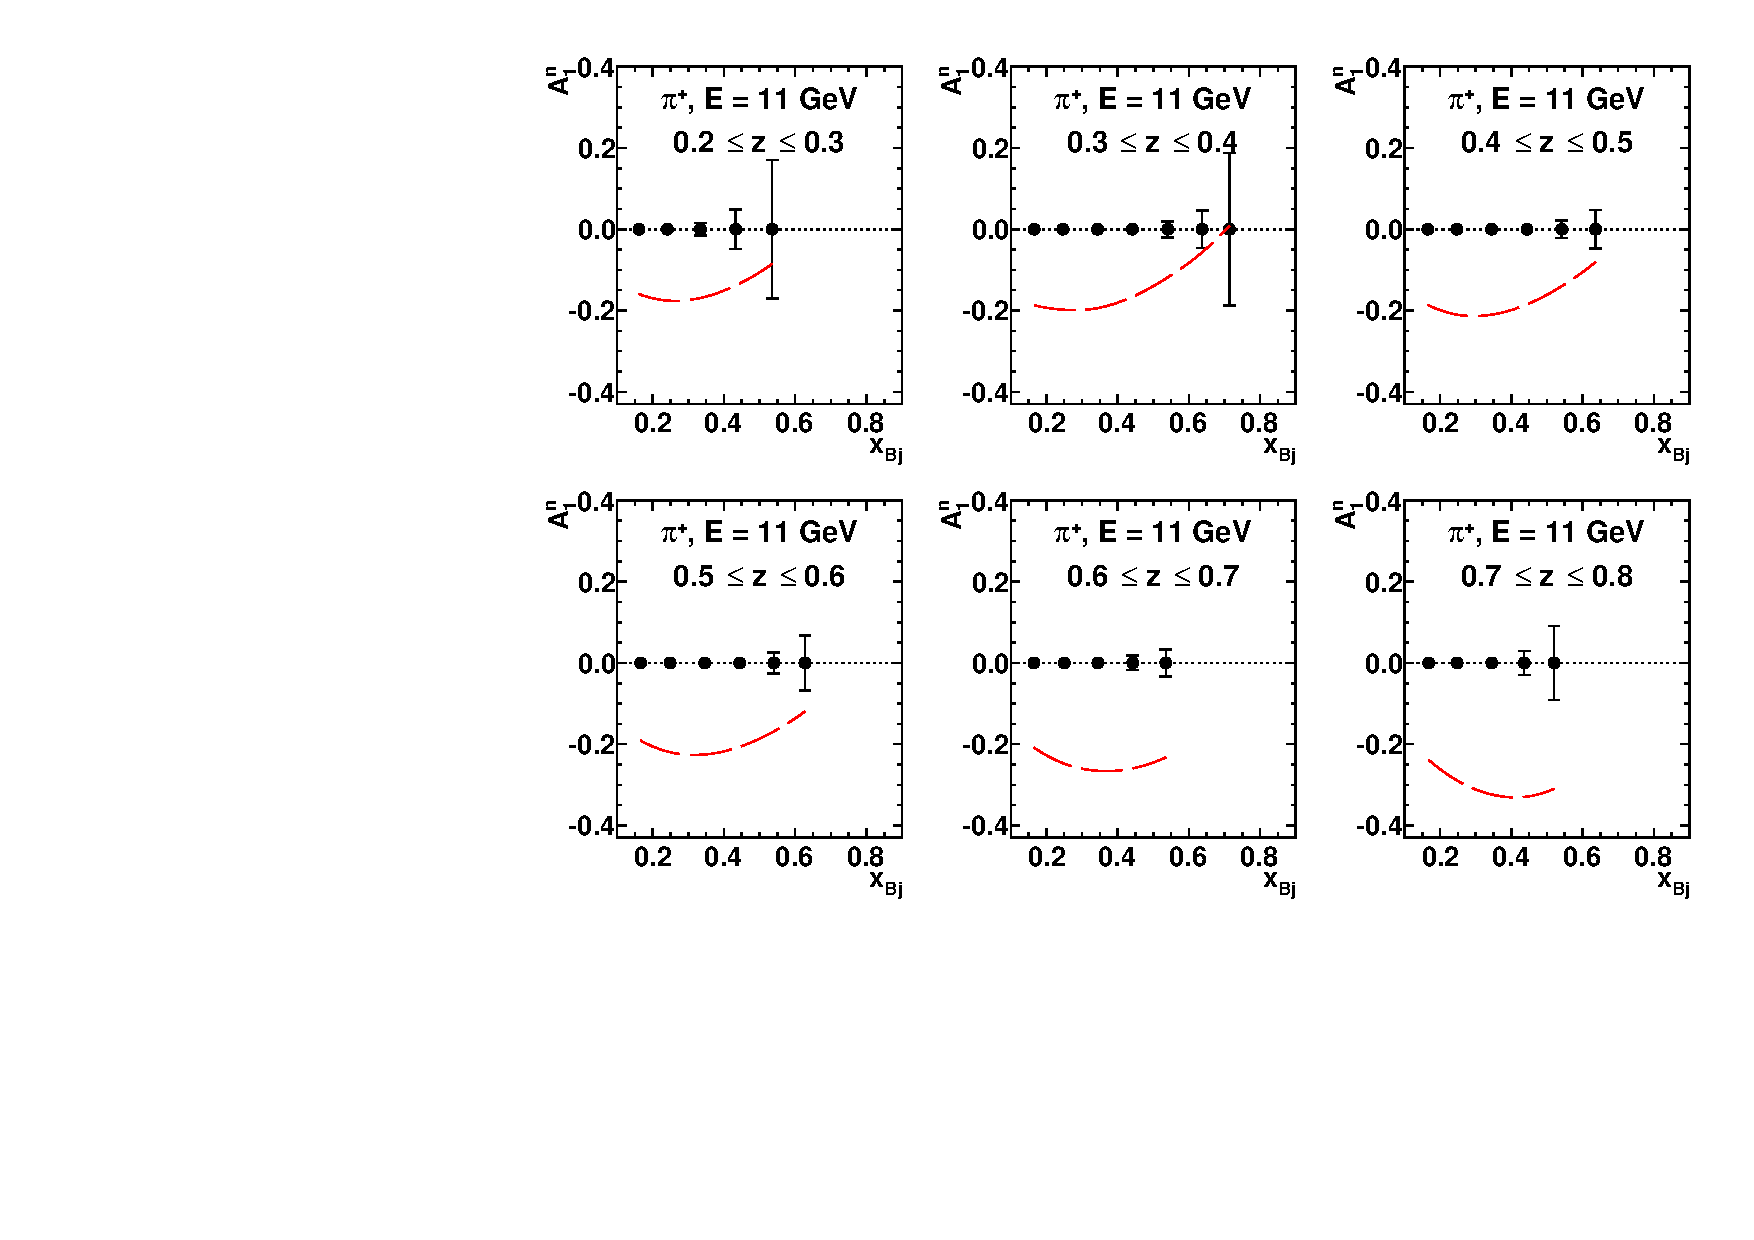
\includegraphics[width=.75\textwidth]{figures/A1n_vs_x_E11_pip.pdf}
  \end{center}
  \caption{\label{A1n_pip_11gev} Projected uncertainties in $A_{1n}^{\pi^+}(x,z)$ from combined 11 GeV running at both SBS angle settings, compared to the predictions of the recent NLO global QCD analysis of DSSV~\cite{DSSVplus}}
\end{figure}

\begin{figure}[h]
  \begin{center}
    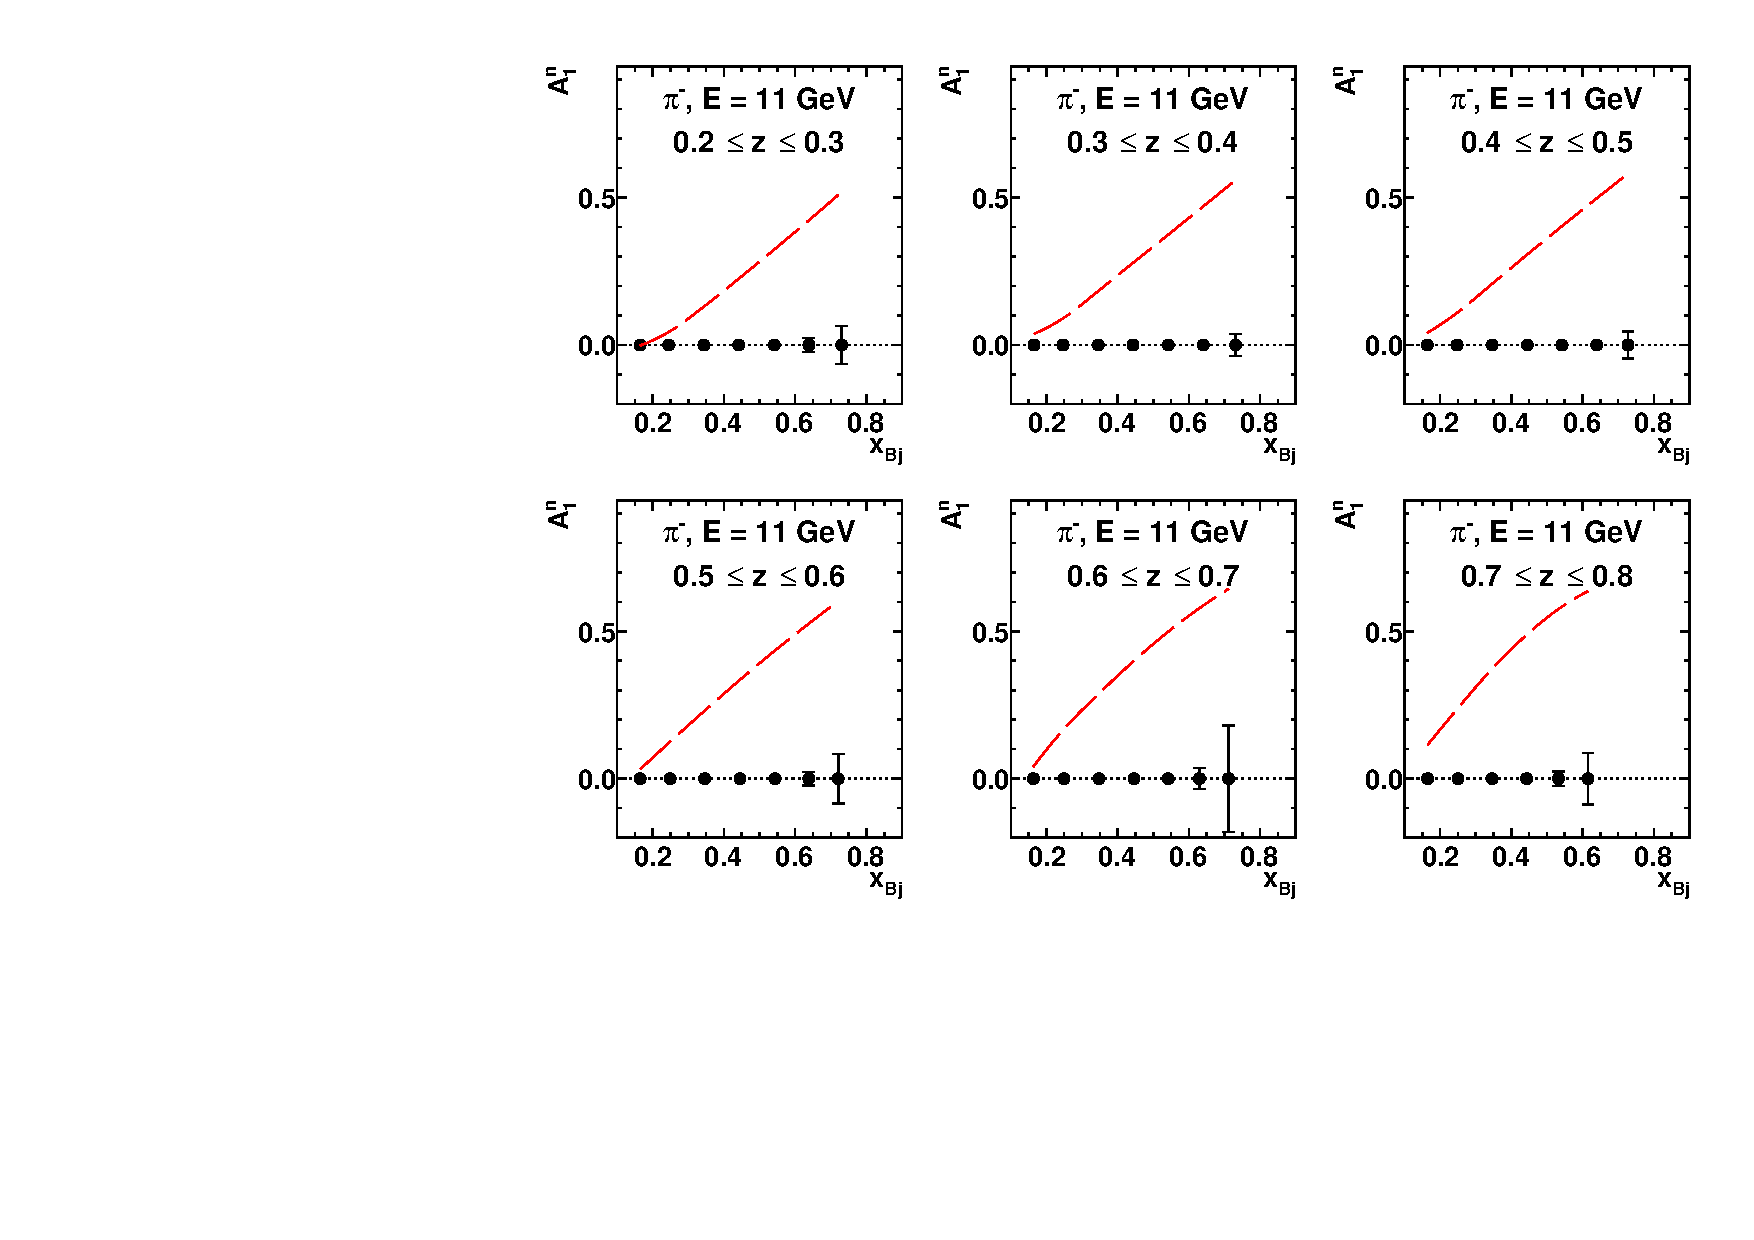
\includegraphics[width=.75\textwidth]{figures/A1n_vs_x_E11_pim.pdf}
  \end{center}
  \caption{\label{A1n_pim_11gev} Projected uncertainties in $A_{1n}^{\pi^-}(x,z)$ from combined 11 GeV running at both SBS angle settings, compared to the predictions of the recent NLO global QCD analysis of DSSV~\cite{DSSVplus}}
\end{figure}


\begin{figure}[h]
  \begin{center}
    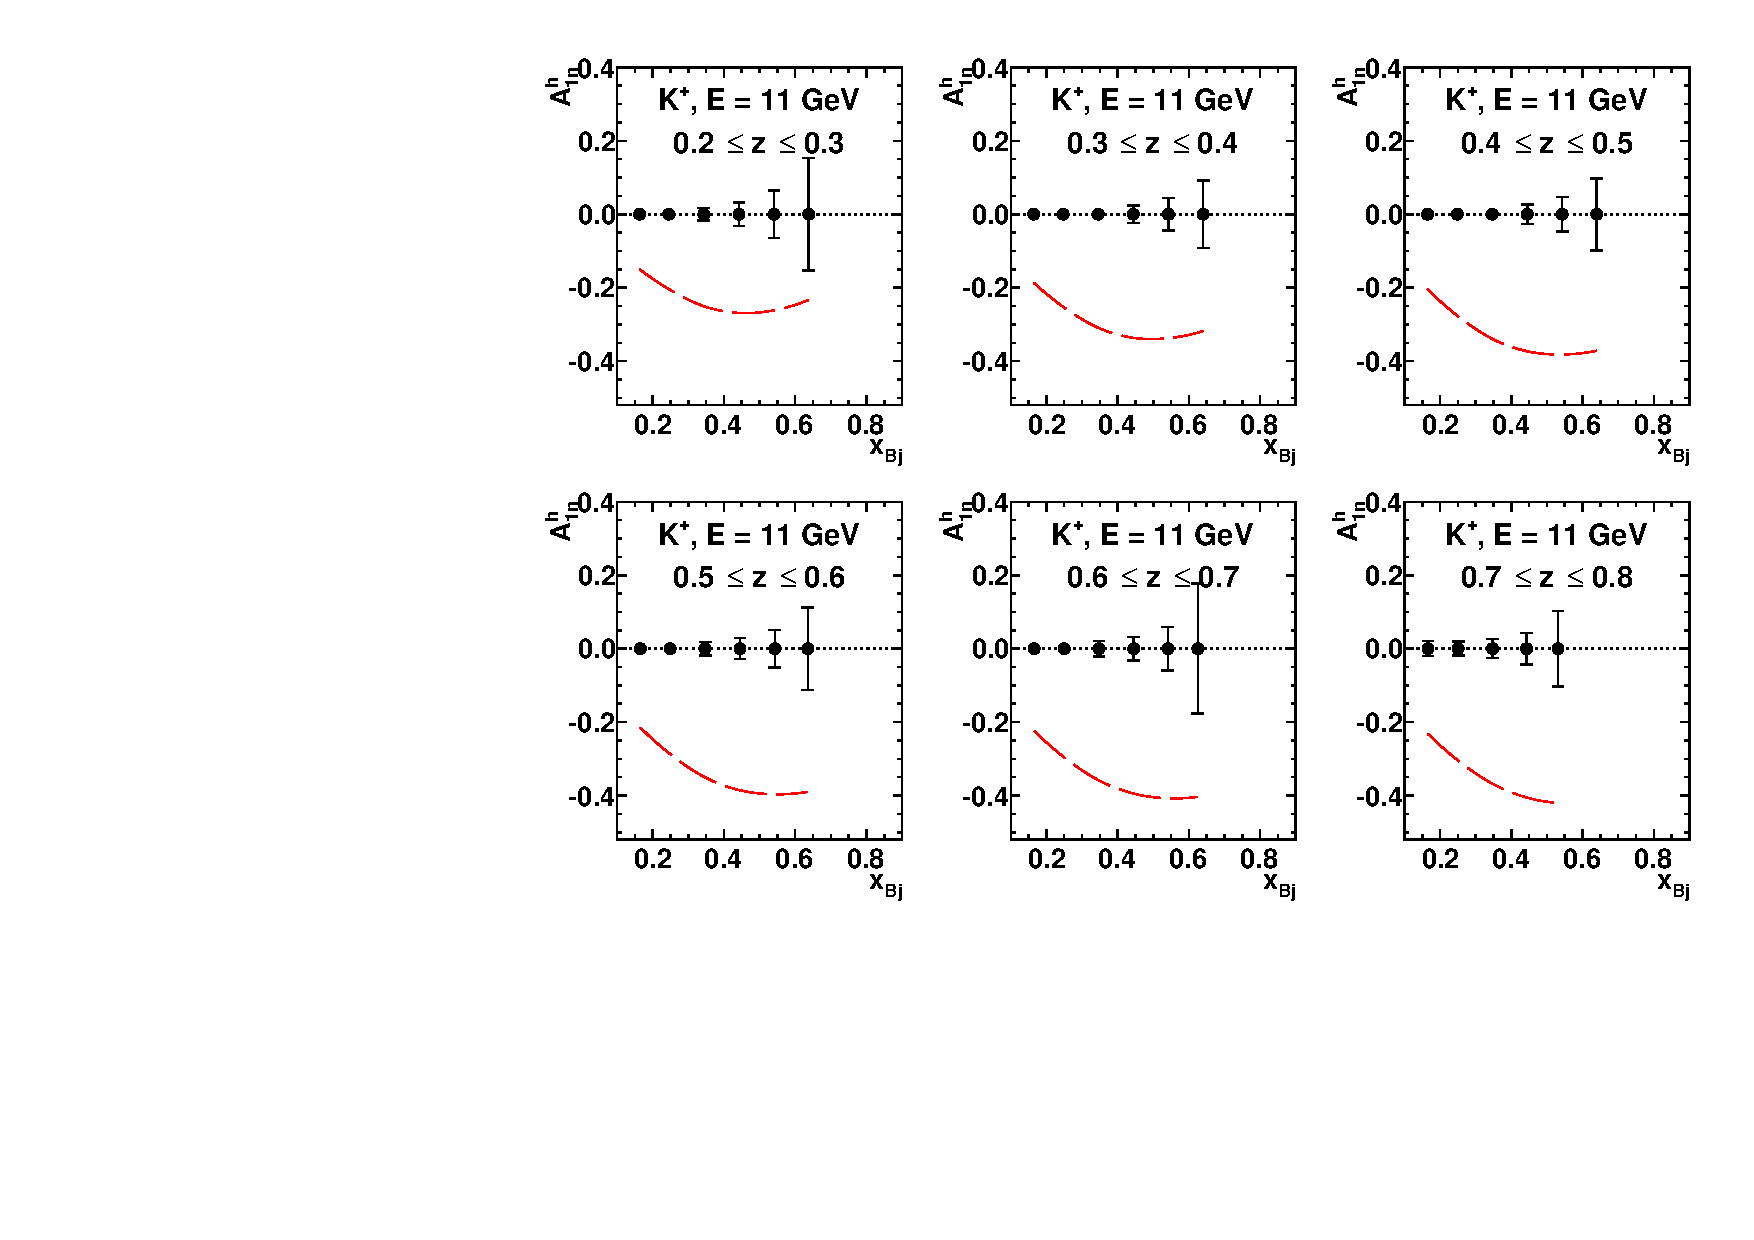
\includegraphics[width=.75\textwidth]{figures/A1n_vs_x_E11_kp.pdf}
  \end{center}
  \caption{\label{A1n_kp_11gev} Projected uncertainties in $A_{1n}^{K^+}(x,z)$ from combined 11 GeV running at both SBS angle settings, compared to the predictions of the recent NLO global QCD analysis of DSSV~\cite{DSSVplus}}
\end{figure}

\begin{figure}[h]
  \begin{center}
    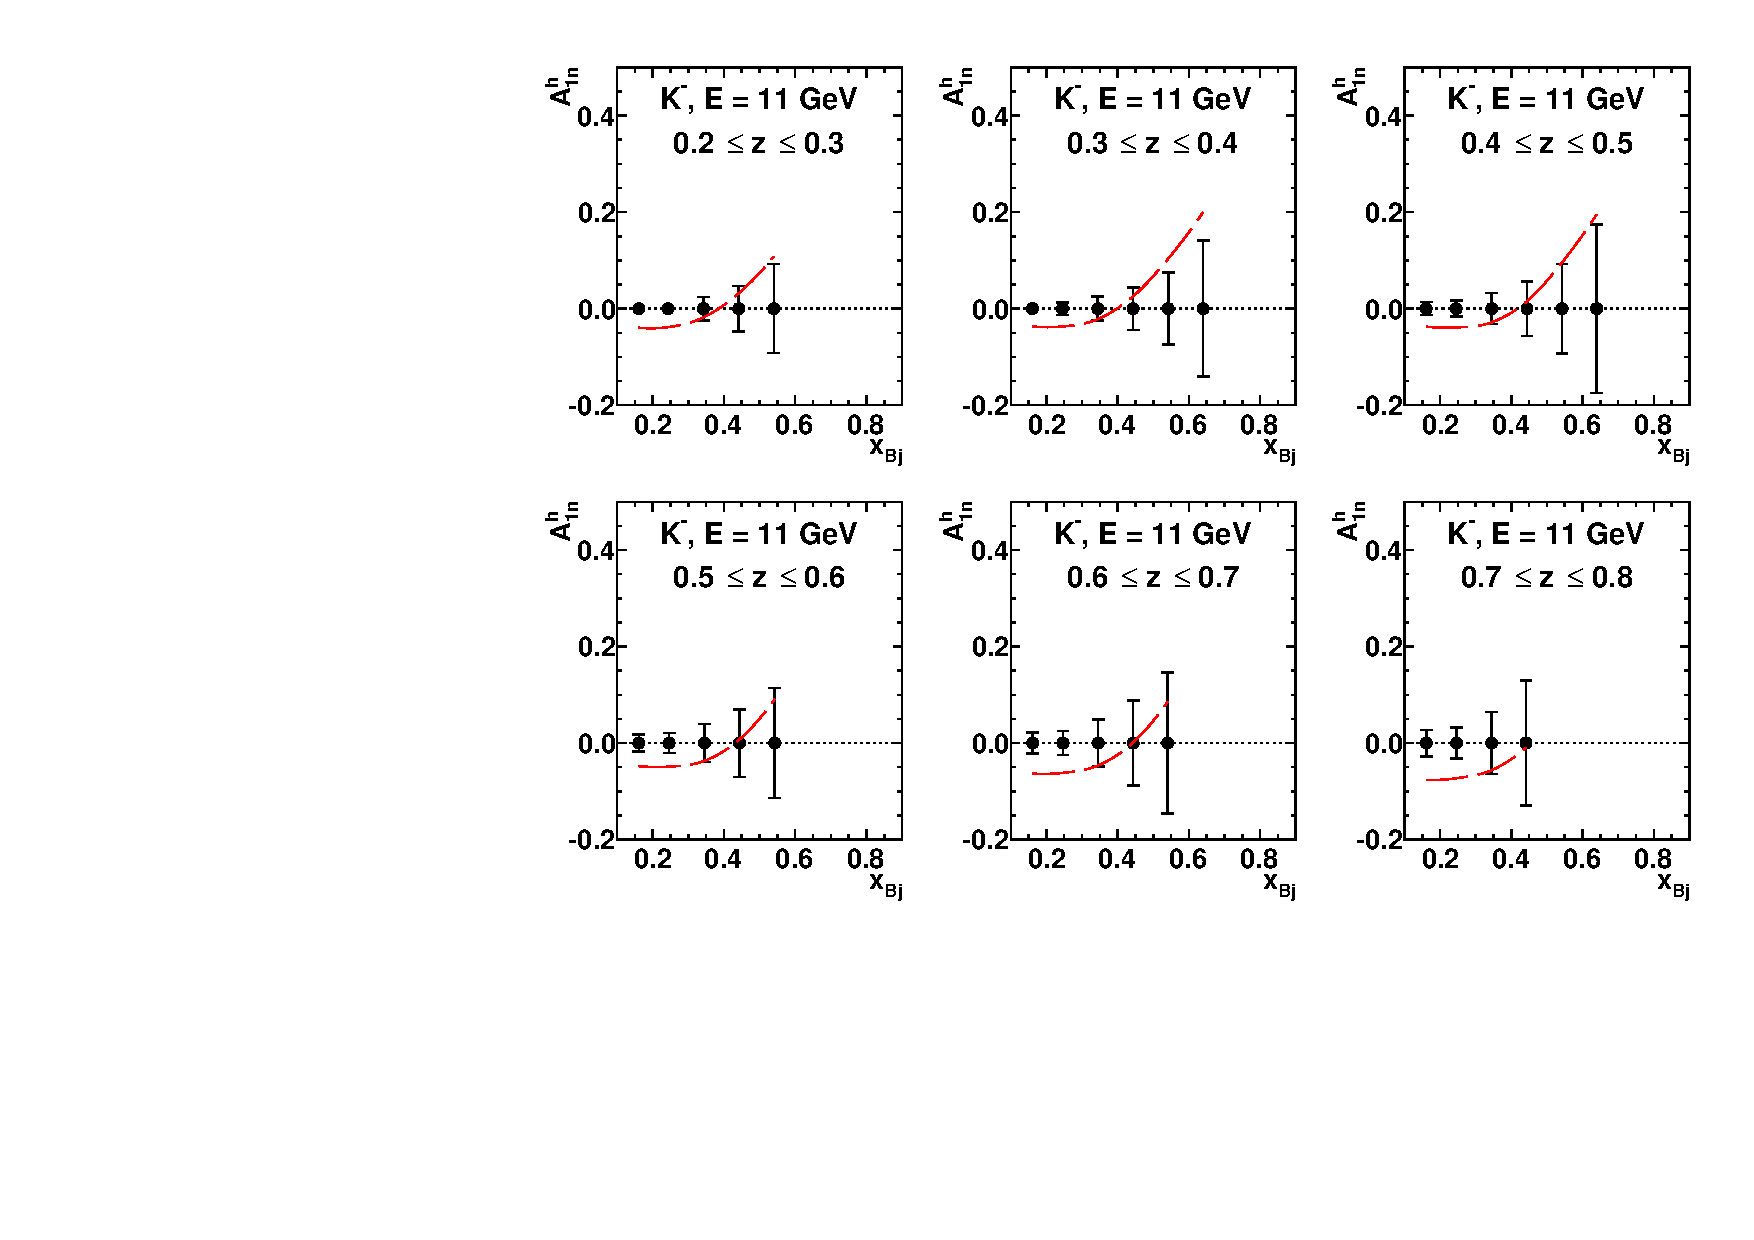
\includegraphics[width=.75\textwidth]{figures/A1n_vs_x_E11_km.pdf}
  \end{center}
  \caption{\label{A1n_km_11gev} Projected uncertainties in $A_{1n}^{K^-}(x,z)$ from combined 11 GeV running at both SBS angle settings, compared to the predictions of the recent NLO global QCD analysis of DSSV~\cite{DSSVplus}}
\end{figure}

\begin{figure}[h]
  \begin{center}
    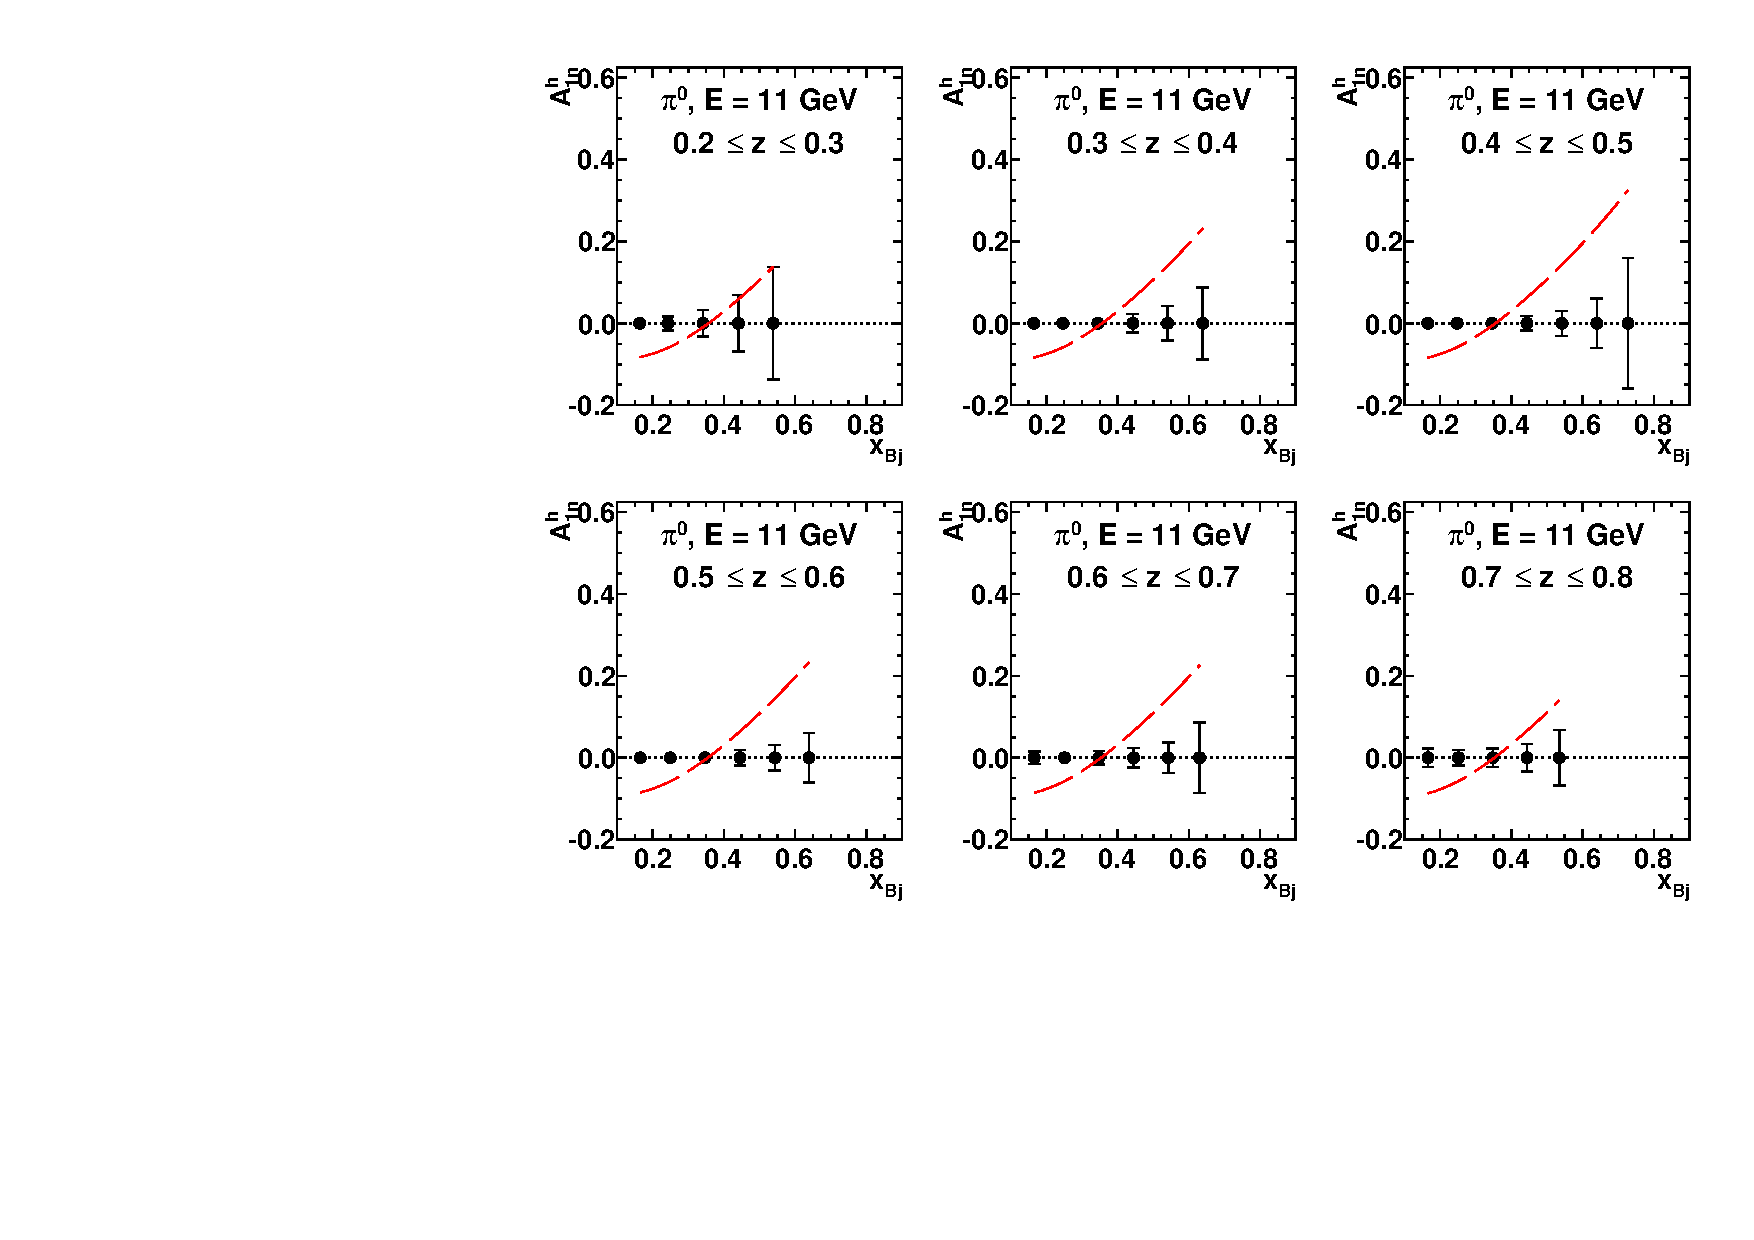
\includegraphics[width=.75\textwidth]{figures/A1n_vs_x_E11_pi0.pdf}
  \end{center}
  \caption{\label{A1n_pi0_11gev} Projected uncertainties in $A_{1n}^{\pi^0}(x,z)$ from combined 11 GeV running at both SBS angle settings, compared to the predictions of the recent NLO global QCD analysis of DSSV~\cite{DSSVplus}}
\end{figure}

\begin{figure}[h]
  \begin{center}
    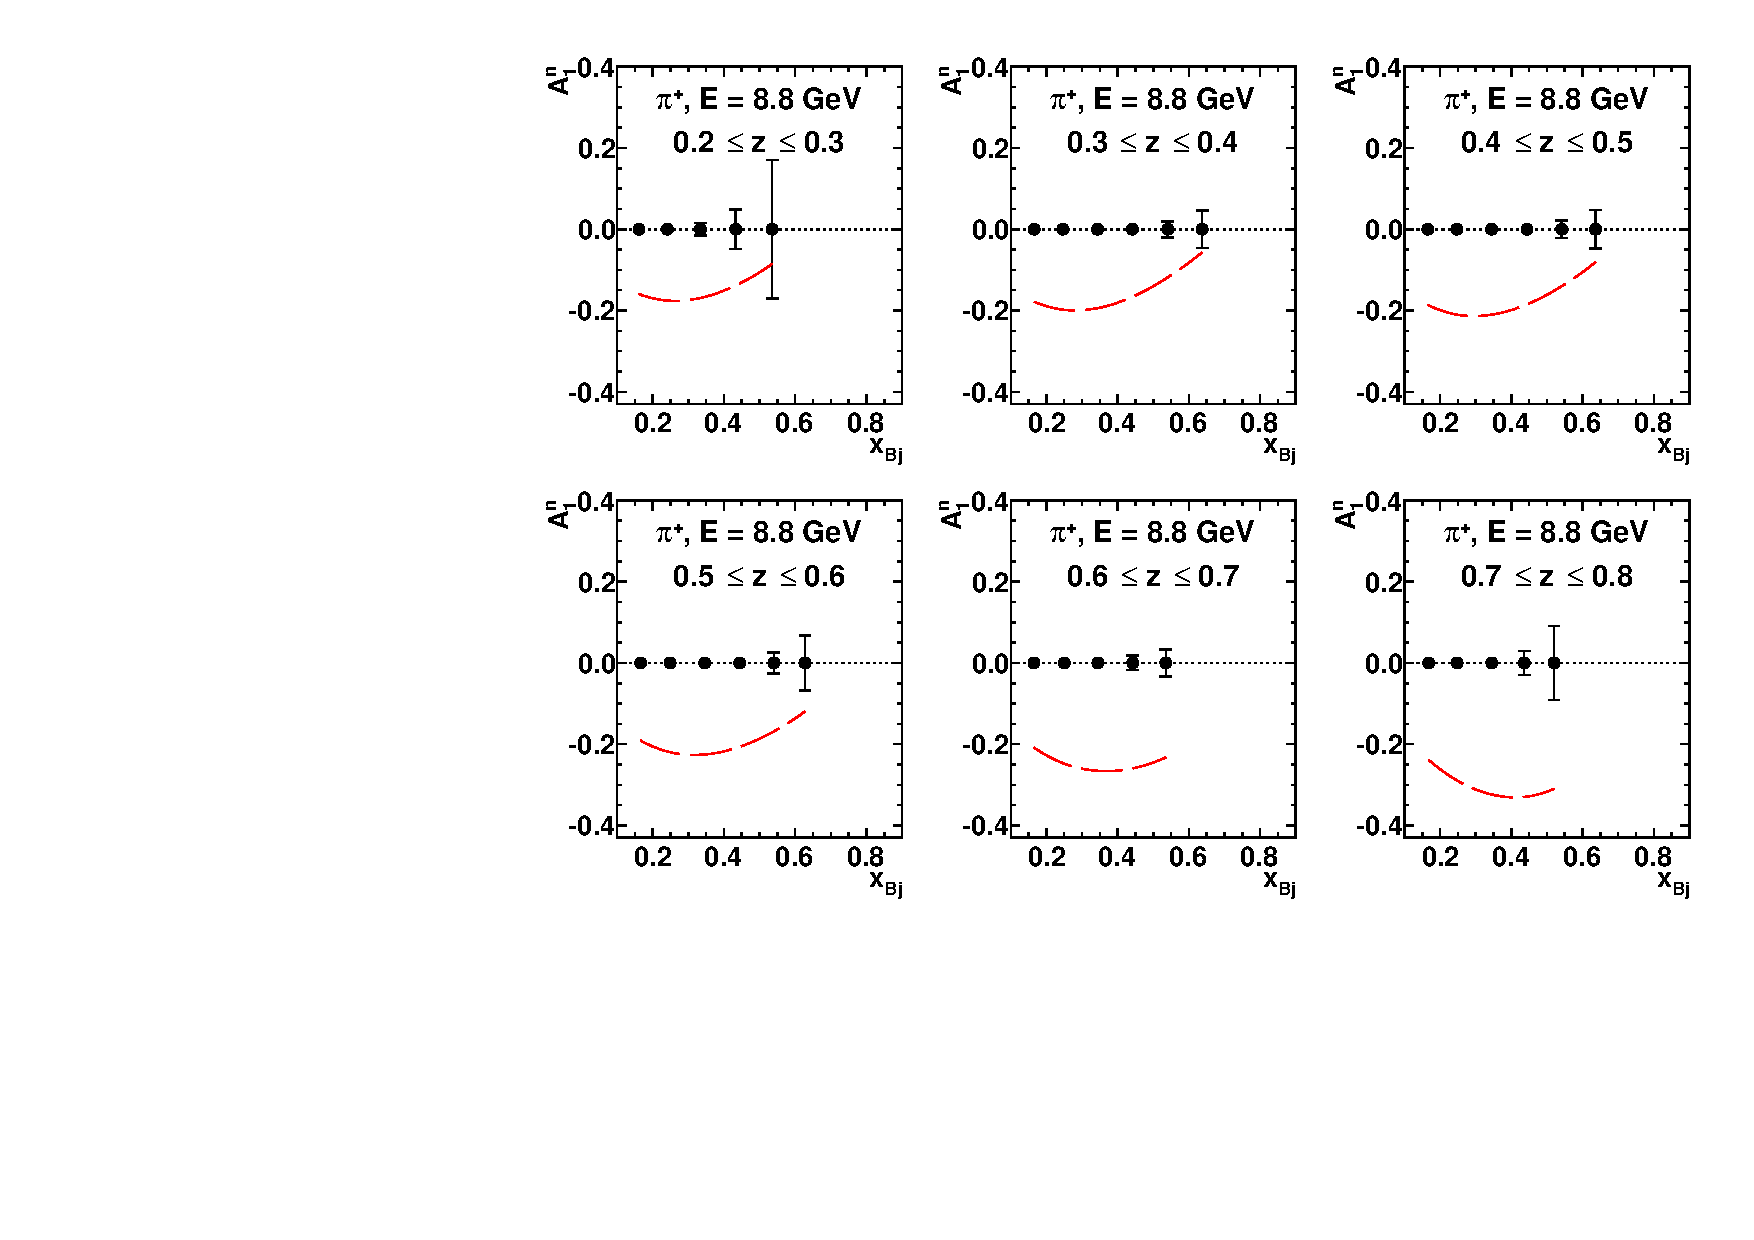
\includegraphics[width=.75\textwidth]{figures/A1n_vs_x_E88_pip.pdf}
  \end{center}
  \caption{\label{A1n_pip_88gev} Projected uncertainties in $A_{1n}^{\pi^+}(x,z)$ from combined 8.8 GeV running at both SBS angle settings, compared to the predictions of the recent NLO global QCD analysis of DSSV~\cite{DSSVplus}}
\end{figure}
\begin{figure}[h]
  \begin{center}
    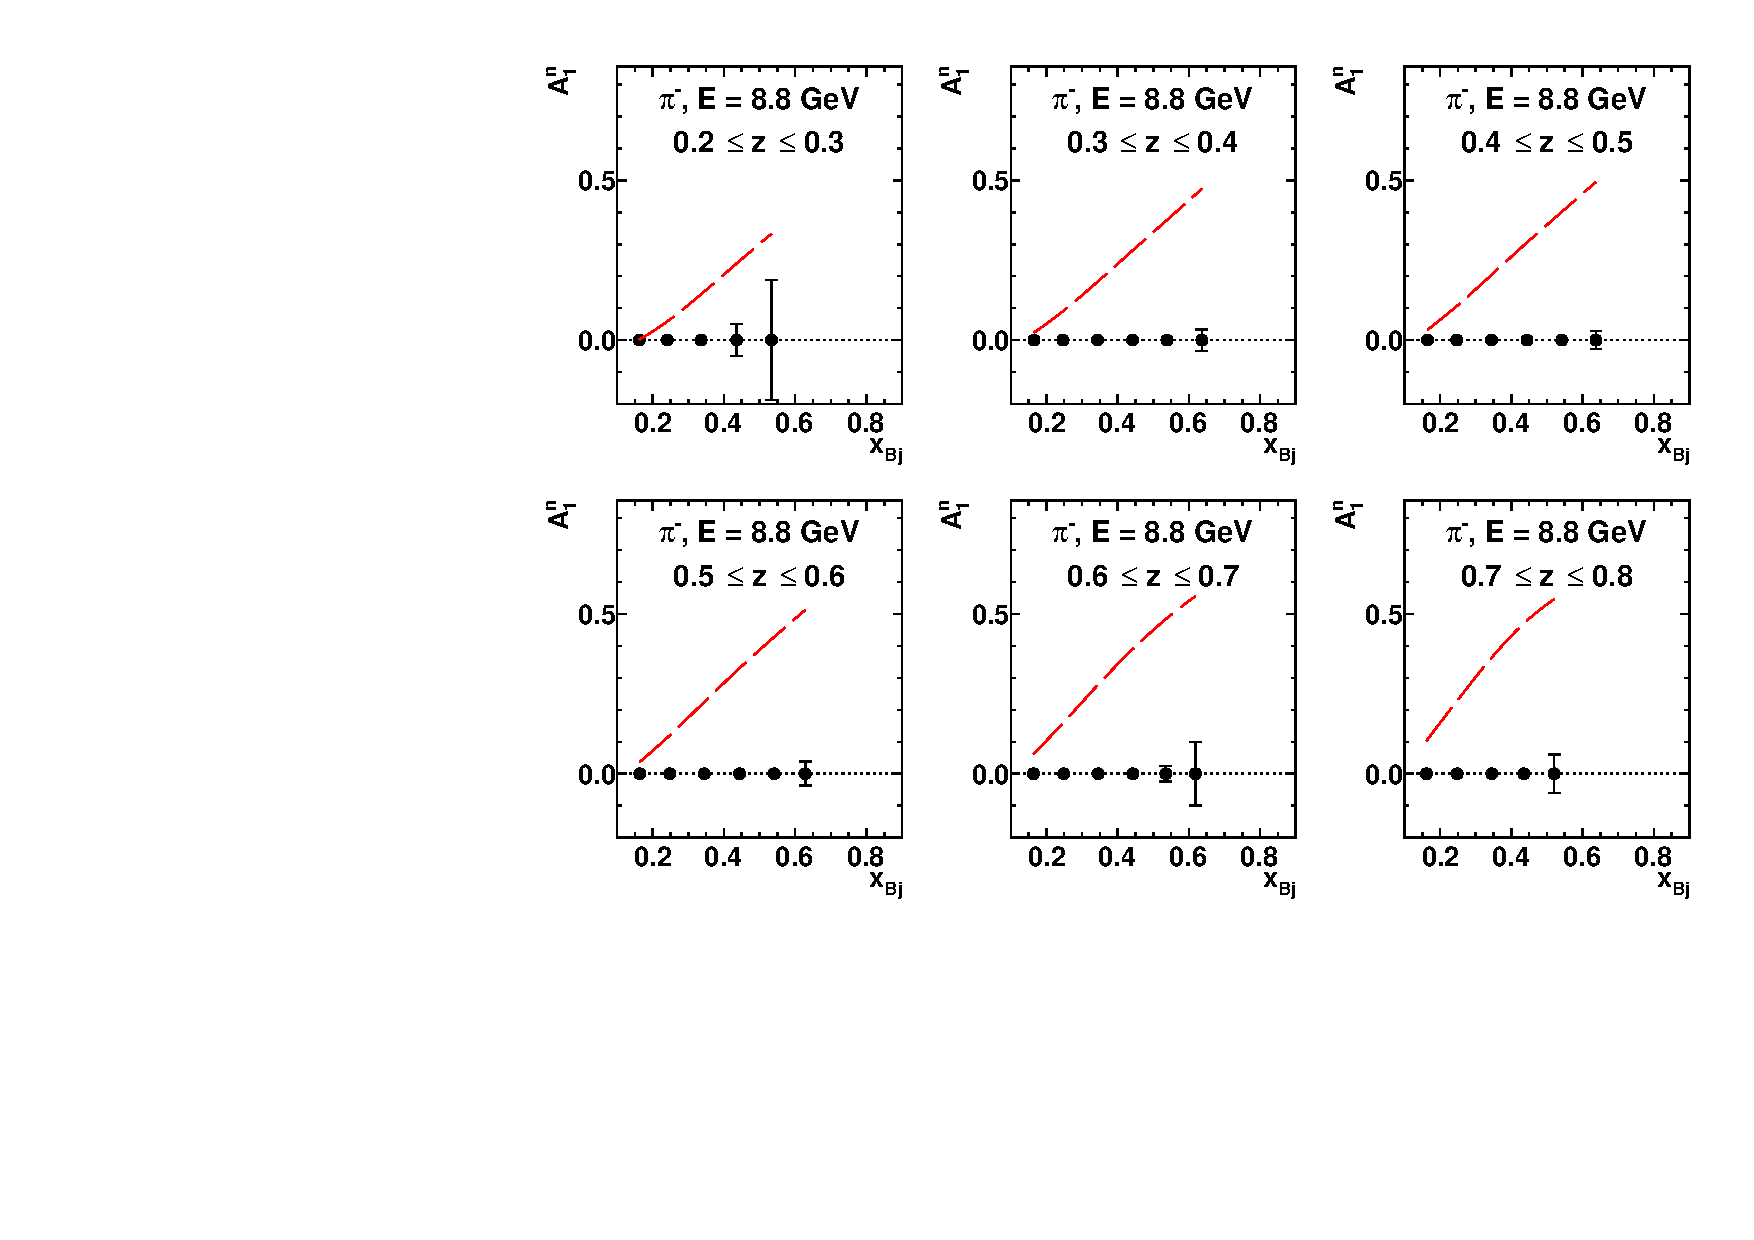
\includegraphics[width=.75\textwidth]{figures/A1n_vs_x_E88_pim.pdf}
  \end{center}
  \caption{\label{A1n_pim_88gev} Projected uncertainties in $A_{1n}^{\pi^-}(x,z)$ from combined 8.8 GeV running at both SBS angle settings, compared to the predictions of the recent NLO global QCD analysis of DSSV~\cite{DSSVplus}}
\end{figure}
\begin{figure}[h]
  \begin{center}
    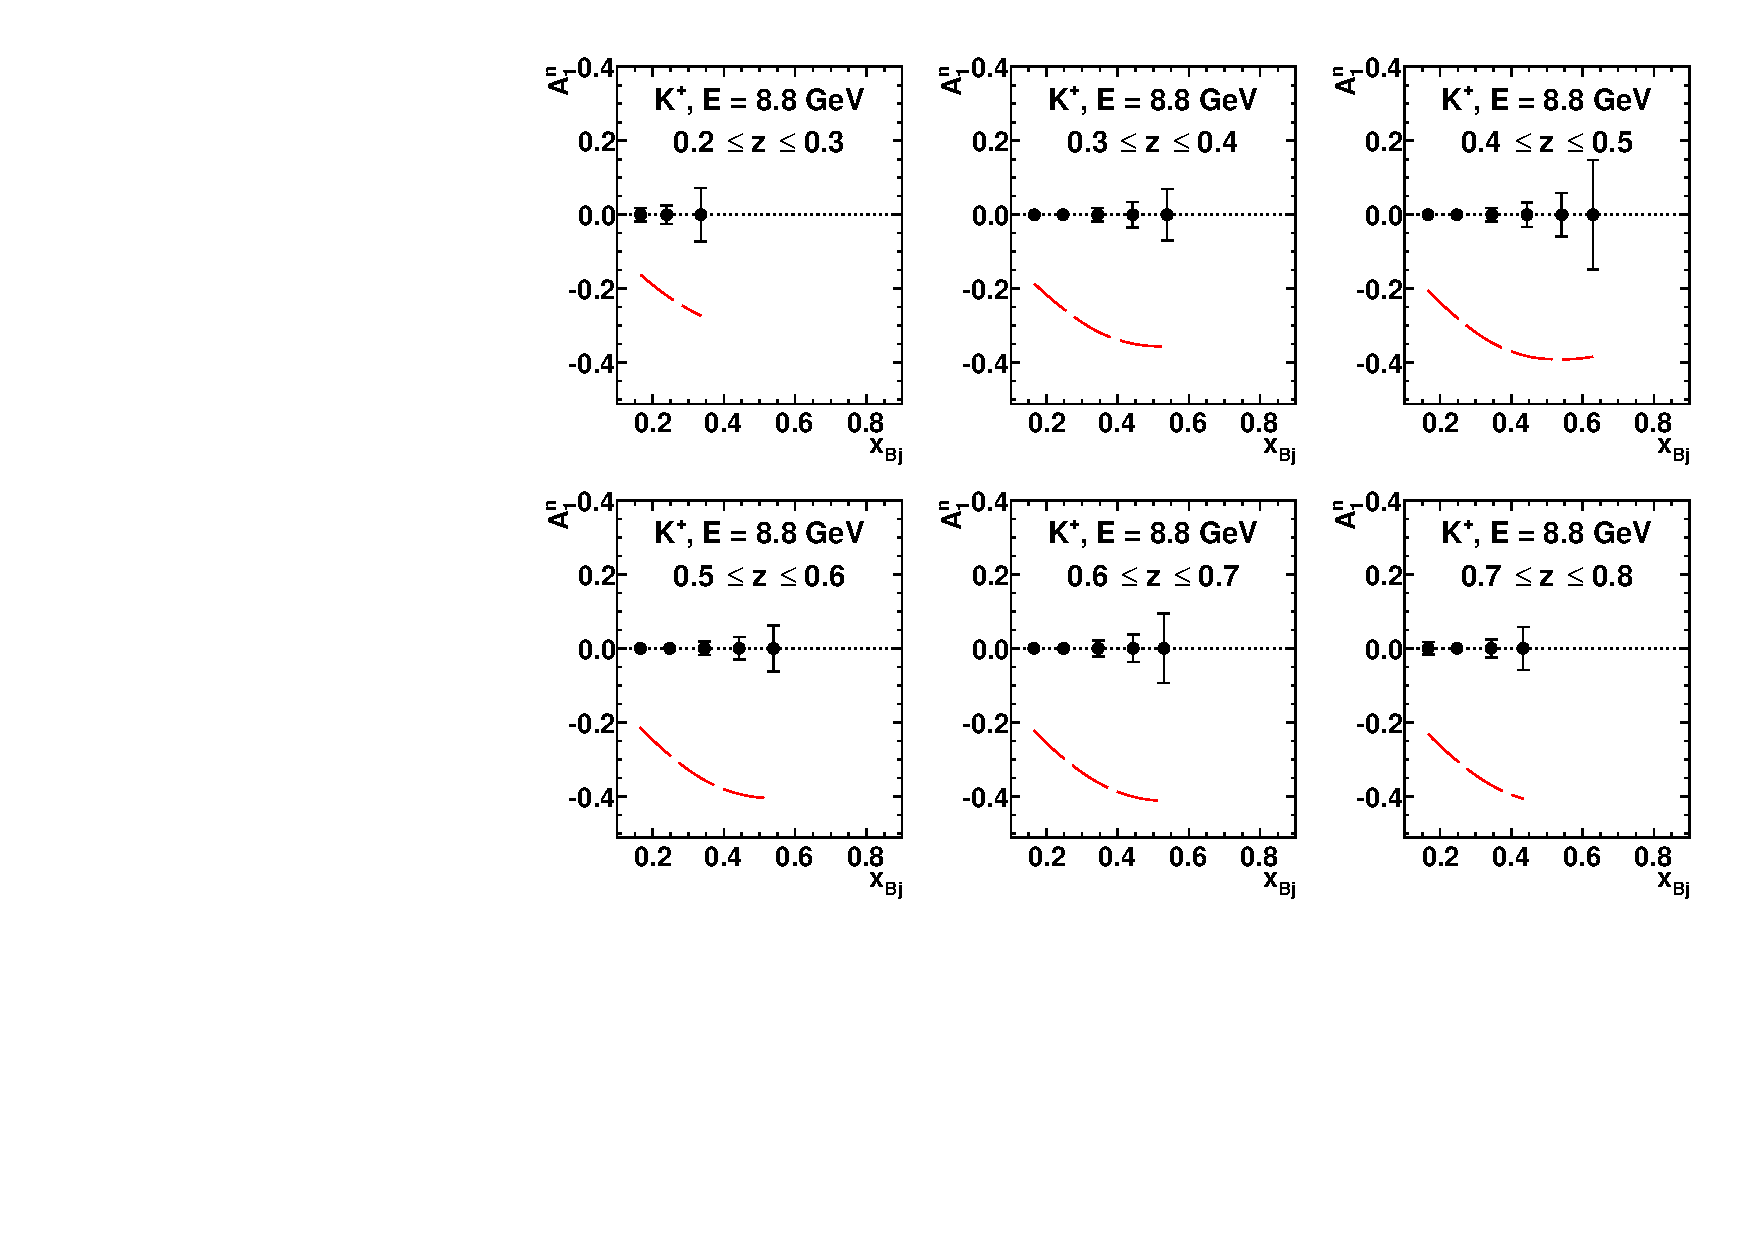
\includegraphics[width=.75\textwidth]{figures/A1n_vs_x_E88_kp.pdf}
  \end{center}
  \caption{\label{A1n_kp_88gev} Projected uncertainties in $A_{1n}^{K^+}(x,z)$ from combined 8.8 GeV running at both SBS angle settings, compared to the predictions of the recent NLO global QCD analysis of DSSV~\cite{DSSVplus}}
\end{figure}
\begin{figure}[h]
  \begin{center}
    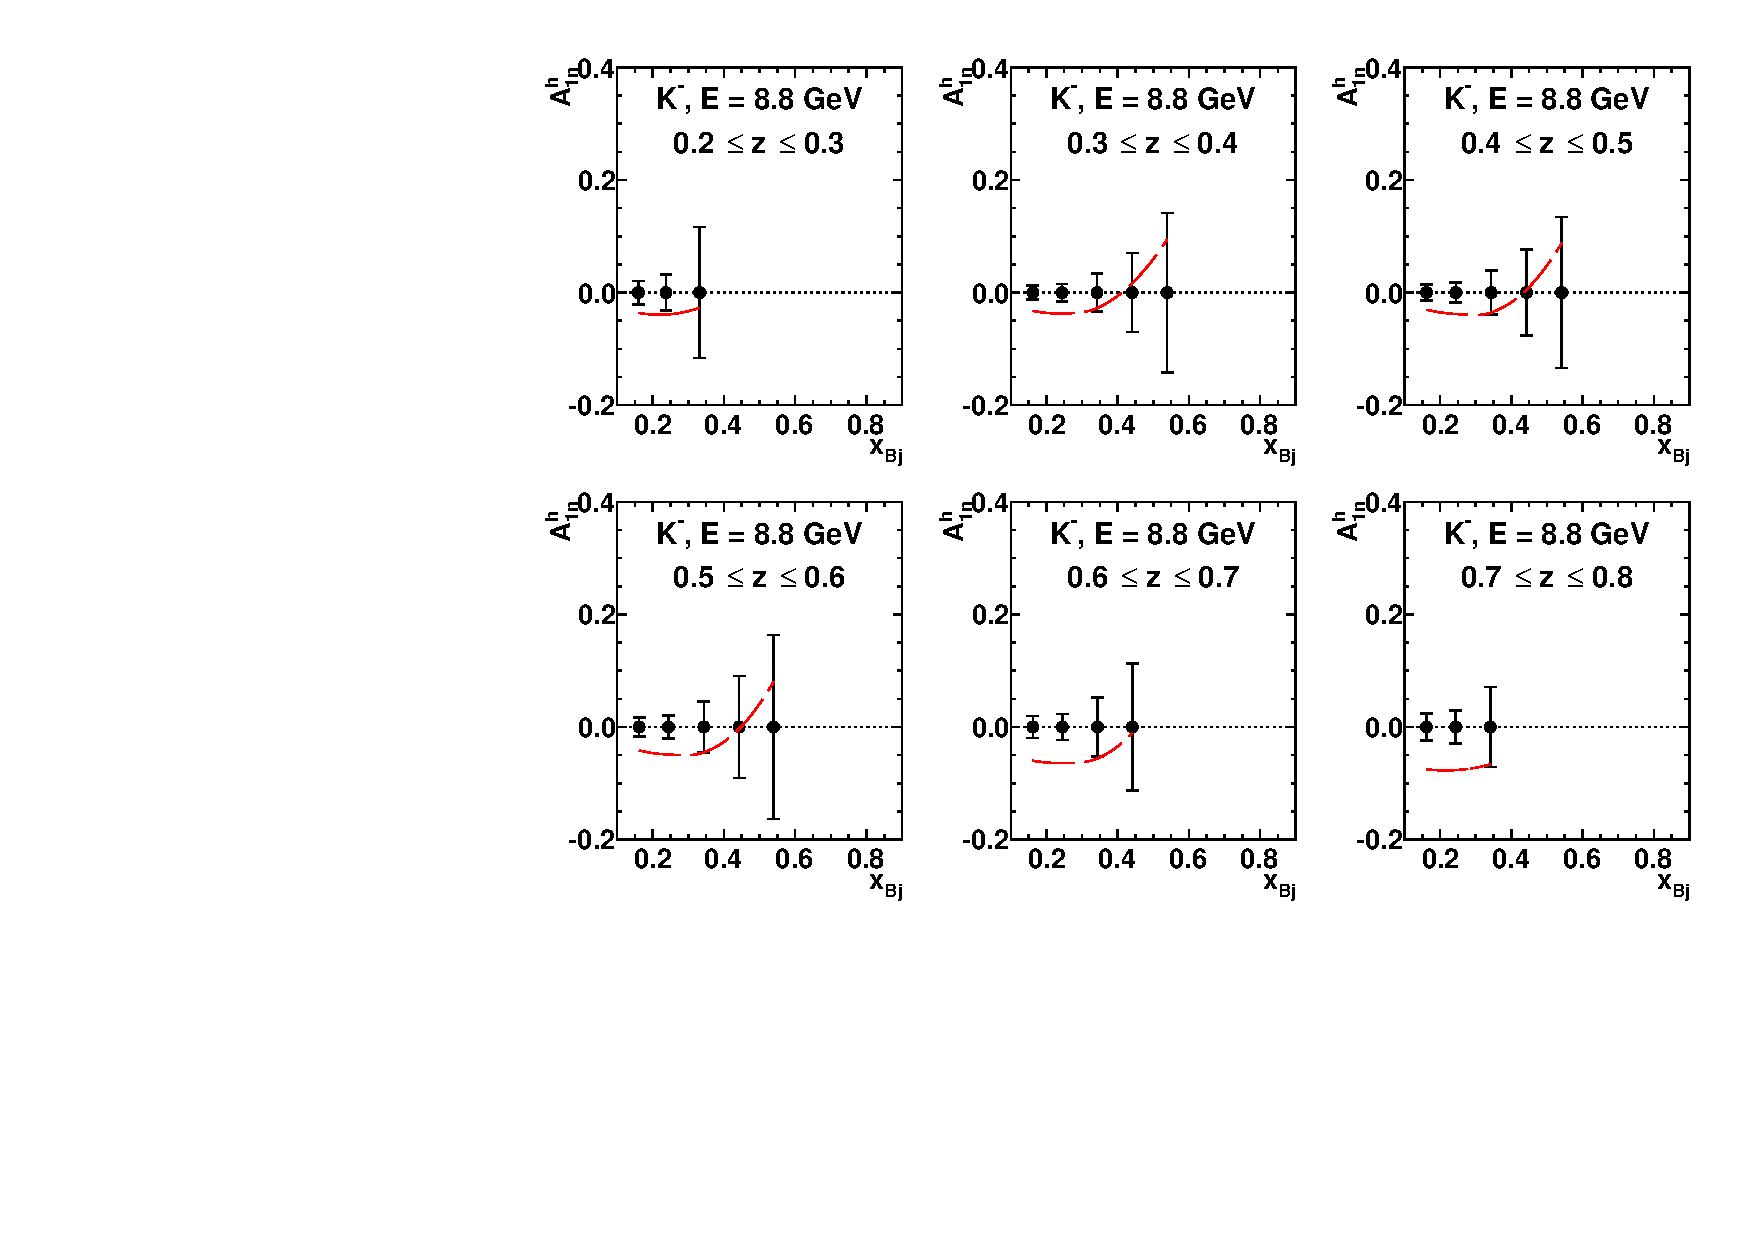
\includegraphics[width=.75\textwidth]{figures/A1n_vs_x_E88_km.pdf}
  \end{center}
  \caption{\label{A1n_km_88gev} Projected uncertainties in $A_{1n}^{K^-}(x,z)$ from combined 8.8 GeV running at both SBS angle settings, compared to the predictions of the recent NLO global QCD analysis of DSSV~\cite{DSSVplus}}
\end{figure}
\begin{figure}[h]
  \begin{center}
    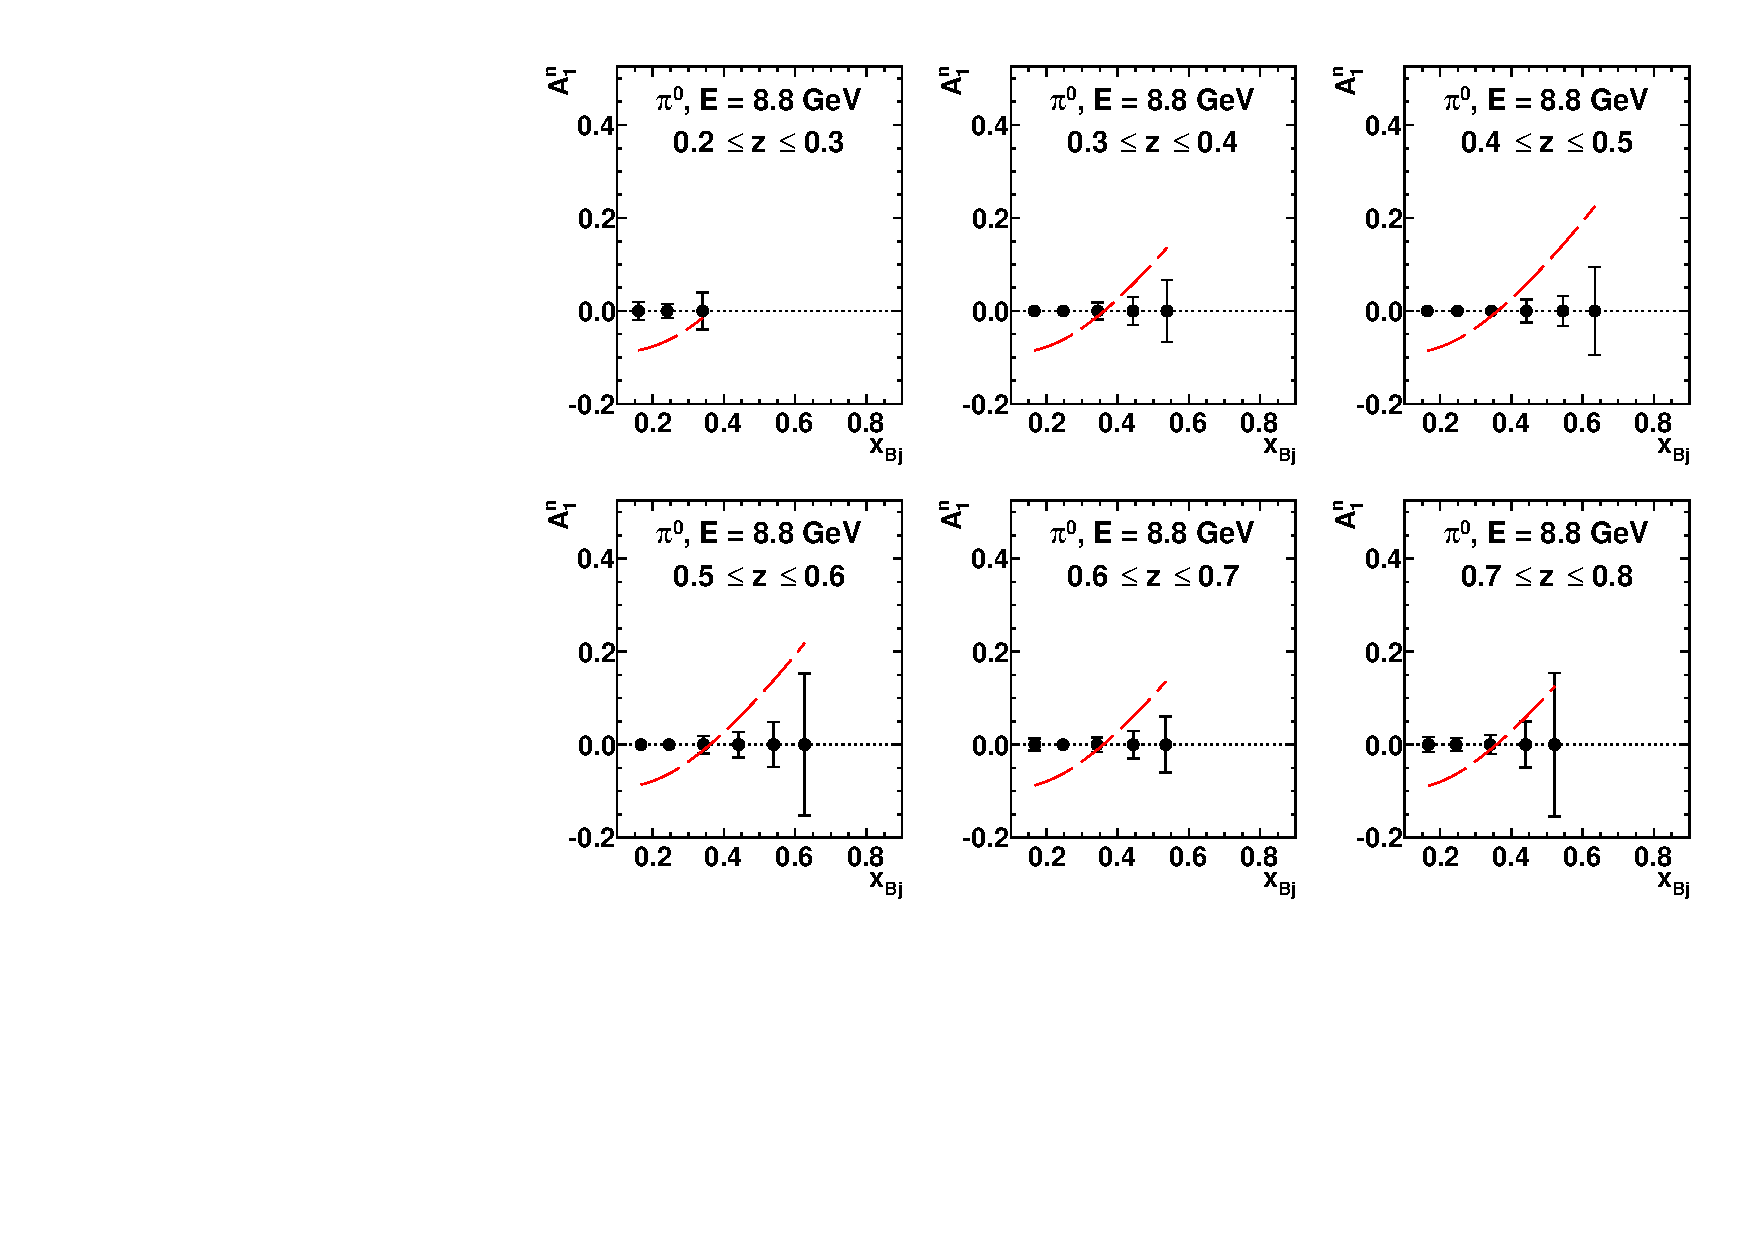
\includegraphics[width=.75\textwidth]{figures/A1n_vs_x_E88_pi0.pdf}
  \end{center}
  \caption{\label{A1n_pi0_88gev} Projected uncertainties in $A_{1n}^{\pi^0}(x,z)$ from combined 8.8 GeV running at both SBS angle settings, compared to the predictions of the recent NLO global QCD analysis of DSSV~\cite{DSSVplus}}
\end{figure}
